\chapter{Hardware}
\label{3_hardware}

Ce chapitre présente toute l'implémentation de la carte électronique qui a été réalisée dans ce projet. On y présente celle-ci avec la description des composants. Le choix de ces composants y est également évoqué.


\section{Introduction}

Après avoir analyser les différents besoin 



\section{Architecture}

Nous désirions utiliser deux processeurs sur la carte électronique. Nous avions donc deux implémentations possibles. Les \autoref{fig:hardware_option1} et \autoref{fig:hardware_option2} illustrent toutes deux ces deux options. La première consiste à utilise un processeur LoRa comme processeur principal du système. C'est à dire un processeur sur lequel la communication LoRa est gérée en plus de la gestion des différents périphériques de la carte. Comme par exemple le GPS, un accéléromètre, etc. Le processeur gérant le Bluetooth serait donc comme un simple périphérique pour le processeur LoRa. Une API doit être mise en place pour faciliter l'échange d'information entre les deux. La deuxième possibilité est d'inverser les rôle des processeurs. Le processeur principal serait celui qui gère les protocoles en 2.4 GHz et communiquant périodiquement avec le processeur LoRa afin d'envoyer et recevoir des données provenant du réseau.

\begin{figure}[ht!]
    \centering
    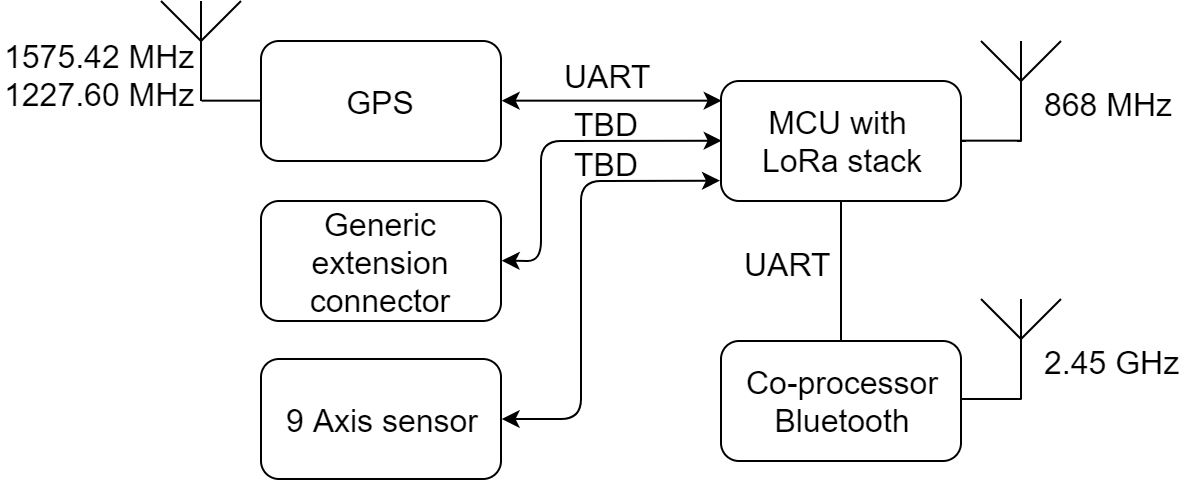
\includegraphics[width=\textwidth]{Figures/hardware/master_onepage_option1.png}
    \caption{Architecture option numéro 1}
    \label{fig:hardware_option1}
\end{figure}

\begin{figure}[ht!]
    \centering
    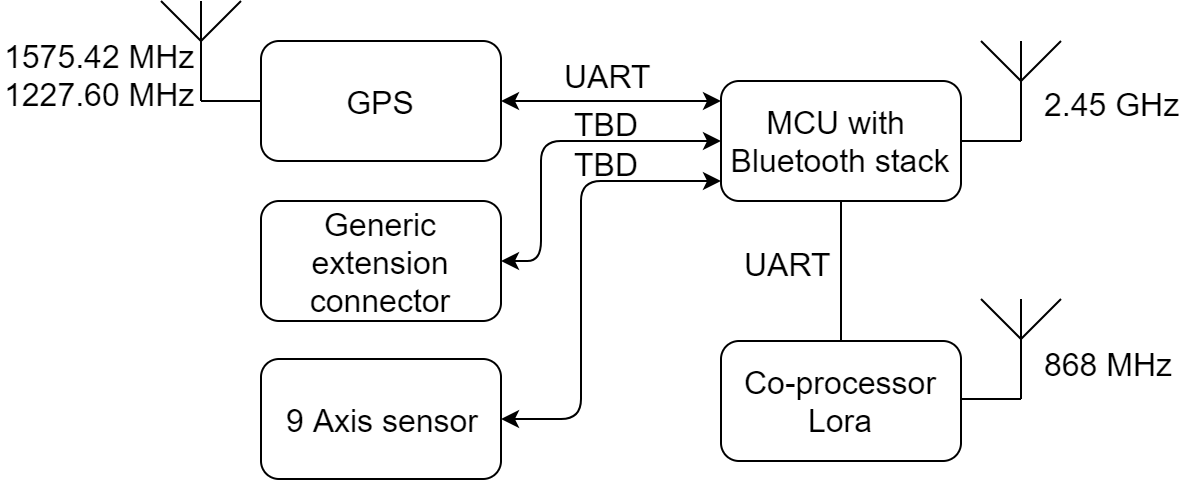
\includegraphics[width=\textwidth]{Figures/hardware/master_onepage_option2.png}
    \caption{Architecture option numéro 2}
    \label{fig:hardware_option2}
\end{figure}

L'architecture choisie est la numéro 2. Nous avons donc tous les périphériques qui sont connectés au processeur s'occupant du Bluetooth. Le processeur avec l'interface LoRa, lui ne s'occupe que de communiquer les évènements de réception de données ainsi que de transférer les messages provenant depuis le processeur 2.4 GHz.

Il est également plus simple de faire une API pour le LoRa, le nombre de données et paramètres configurables sont moins importants que dans le cas des communications 2.4GHz. Si on souhaite donc faire une API entre les deux processeur, il est nécessaire de tenir compte de la complexité de ceux-ci. Les accès LoRa sont également plus ponctuelles. Le nombre de paquets envoyé par heures sont très faibles à comparer à ce qui est réalisable en 2.4 GHz. On peut ainsi faire en sorte que le processeur soit en mode très basse consommation en attendant une commande de la part du processeur principal ou la réception d'un paquet LoRa sur son antenne.


\section{Choix du matériel}

Cette section a pour rôle d'expliquer les différents choix effectués pour les composants présents sur la DevBox. 

\subsection{Microcontrôleur}
\label{subsect:microcontroleur}

Pour choisir quel microcontrôleur était l'idéal pour le cahier des charges un comparatif approfondis a été effectué. Ce comparatif est visible sur le \autoref{mcu_table}. Donc premièrement, un des point qui a été retenu a été le type de protocole qui est supporté par le processeur. Le Bluetooth Low Energy étant un prérequis, cela nous a permis de faire en sorte d'avoir un premier filtre. C'est pour cela que tous les microcontrôleur affichés disposent tous cette fonctionnalité. Néanmoins, dans le Bluetooth Low Energy on y trouve la norme 4.2 qui a été annoncée le 2 décembre 2014 \cite{Bluetoot59:online} et la norme 5.0 annoncée elle le 16 juin 2016. Cette dernière n'était malheureusement pas encore parfaitement supportée par tous les fabricants de microcontrôleur. Comme expliqué précédemment sous la \autoref{sec_2_4_GHz}, une simple mise à jour logicielle permet de passer un microcontrôleur en Bluetooth 5.0, du moins, en garantissant les fonctionnalité primordiales du protocole. Les microcontrôleur affichés dans le tableau disposait, à la date du 1 octobre 2017, que des fonctionnalités listées.

Après le Bluetooth, le deuxième type de protocole est le IEEE 802.15.4 \cite{IEEE802137:online}. Ce standard IEEE n'est pas un protocol en tant que tel, mais c'est un modèle qui est respecté par plusieurs ptotocoles du commerce. On trouve différents protocoles qui sont utilisable avec ce standard, comme le ZigBee, WirelessHART, MiWi, SNAP, ou encore Thread. Ce standard est de plus en plus utilisé pour la domotique. Il permet de facilement créer des réseaux maillés permettant ainsi une grande couverture de l'habitation.

Un dernier moyen de communication en dessous d'un GHz. Si le processeur supporte cela, ça peut être un avantage. Néanmoins, la communication dans cette plage de fréquence a quelques désavantages, en commençant par la taille de l'antenne qu'il faut utiliser. La consommation du processeur est également affectée, pouvant atteindre jusqu'à 100 mA (cf. EFR32M datasheet).

LoRa rentre dans cette catégorie, mais uniquement les processeurs fournis par Semtech peuvent implémenter la modulation. Ils ne sont à l'heure actuelle pas assez évolués pour pouvoir être utilisé comme unique processeur gérant à la fois du 2.4 GHz avec en parallèle une interface LoRa (868 ou 433 MHz).

On a ensuite l'aspect consommation qui rentre en jeu. Afin d'être le plus proche possible en terme de comparaison, la consommation en émission à été retenu pour la fréquence de 2.4 GHz avec une puissance de 0 dBm en sortie. Plus cette consommation est faible et plus notre système aura la possibilité d'être autonome grâce à sa batterie. 

Finalement, les deux derniers points à retenir sont la taille des mémoires (RAM et Flash), qui selon leur taille nous permettront de faire un programme plus complexe et le coût à l'unité du microcontrôleur. Les prix ont été sélectionné pour une seule unité sur le site d'achat Mouser\footnote{\url{http://www.mouser.ch/}} Suisse. 

Après

Le microcontrôleur retenu a donc été le KW41Z de NXP. Celui-ci a été initialement développer par l'entreprise Freescale qui depuis le lancement de ce produit a été rachetée par NXP. 


\begin{sidewaystable}[!ht]
\centering
\caption{Table}
\label{tab:mcu_table}
\begin{tabular}{|l|l|l|c|c|c|c|l|l|c|c|l|}
\hline
\multicolumn{1}{|c|}{\textbf{Manufacturer}} & \multicolumn{1}{c|}{\textbf{Model}} & \multicolumn{1}{c|}{\textbf{CPU}} & \textbf{\begin{tabular}[c]{@{}c@{}}BLE\\ 4.2\end{tabular}} & \textbf{\begin{tabular}[c]{@{}c@{}}BLE\\ 5.0\end{tabular}} & \textbf{\begin{tabular}[c]{@{}c@{}}IEEE\\     802.15.4\end{tabular}} & \textbf{\begin{tabular}[c]{@{}c@{}}Sub\\     1GHz\end{tabular}} & \multicolumn{1}{c|}{\textbf{\begin{tabular}[c]{@{}c@{}}Receive \\     Current\end{tabular}}} & \multicolumn{1}{c|}{\textbf{\begin{tabular}[c]{@{}c@{}}Transmit\\ Current \\ (@ 2.4Ghz, \\ @ 0dBm)\end{tabular}}} & \textbf{\begin{tabular}[c]{@{}c@{}}Flash/\\     SRAM\end{tabular}} & \textbf{Disponibility} & \multicolumn{1}{c|}{\textbf{Price}} \\ \hline
NXP & KW41Z & \begin{tabular}[c]{@{}l@{}}Cortex\\ M0+\end{tabular} & Yes & No & Yes & No & 6.8 mA & 6.1 mA & \begin{tabular}[c]{@{}c@{}}512 kB\\ / 128 kB\end{tabular} & Yes & 6.34 CHF \\ \hline
NXP & QN908x & \begin{tabular}[c]{@{}l@{}}Cortex\\ M4F\end{tabular} & Yes & Yes & No & No & 3.4 mA & 3.4 mA & \begin{tabular}[c]{@{}c@{}}512 kB\\ / 128 kB\end{tabular} & Yes & 5.87 CHF \\ \hline
\begin{tabular}[c]{@{}l@{}}Texas\\     Instrument\end{tabular} & CC2650 & \begin{tabular}[c]{@{}l@{}}Cortex\\ M3\end{tabular} & Yes & No & Yes & No & 6.2 mA & 6.8 mA & \begin{tabular}[c]{@{}c@{}}128 kB\\ / 128 kB\end{tabular} & Yes & 6.34 CHF \\ \hline
\begin{tabular}[c]{@{}l@{}}Texas\\     Instrument\end{tabular} & CC2640R2F & \begin{tabular}[c]{@{}l@{}}Cortex\\ M3\end{tabular} & Yes & Yes & No & No & 6.1 mA & 7.0 mA & \begin{tabular}[c]{@{}c@{}}128 kB\\ / 20 kB\end{tabular} & Yes & 6.34 CHF \\ \hline
\begin{tabular}[c]{@{}l@{}}Nordic \\     Semiconductor\end{tabular} & NRF52832 & \begin{tabular}[c]{@{}l@{}}Cortex\\ M4F\end{tabular} & Yes & Yes & No & No & 5.4 mA & 5.3 mA & \begin{tabular}[c]{@{}c@{}}512 kB\\ / 64 kB\end{tabular} & Yes & 5.51 CHF \\ \hline
\begin{tabular}[c]{@{}l@{}}Nordic \\     Semiconductor\end{tabular} & NRF52840 & \begin{tabular}[c]{@{}l@{}}Cortex\\ M4F\end{tabular} & Yes & Yes & Yes & No & N/A & N/A & \begin{tabular}[c]{@{}c@{}}1MB /\\     256 kB\end{tabular} & No & N/A \\ \hline
Silicon Labs & \begin{tabular}[c]{@{}l@{}}EFR32M\\ G12P433\\ F1024GL125\end{tabular} & \begin{tabular}[c]{@{}l@{}}Cortex\\ M4F\end{tabular} & Yes & Yes & Yes & Yes & 9.3 mA & 9.5 mA & \begin{tabular}[c]{@{}c@{}}1MB /\\     256 kB\end{tabular} & Yes & 13.5 CHF \\ \hline
\end{tabular}
\end{sidewaystable}



\subsection{Alimentation et batterie}

Le système doit pouvoir être autonome, afin de garantir cela, une batterie peut être ajoutée. La capacité de cette batterie reste au choix de l'utilisateur. 

L'utilisateur peut recharger la batterie à l'aide du connecteur micro-USB présent sur la carte. 


L'aspect autonomie peut être encore plus poussé en connectant un panneau solaire directement sur la carte. Celui-ci a son propre connecteur dédié en entrée. Ce panneau permet ainsi de directement charger la batterie qui fournira à son tour la tension pour le système. 

Pour gérer la tension élevée du panneau solaire un circuit intégré nommé BQ24210\footnote{\url{http://www.ti.com/product/BQ24210}} est utilisé. Ce dernier s'occupe directement de la recharge de la batterie supportant en entrée jusqu'à 20V de tension. Il est capable de fournir jusqu'à 800 mA à la batterie, tout en protégeant celle-ci en cas de surtension. Il accepte également la possibilité de recharger avec une tension de 5V, permettant ainsi la recharge directement depuis une prise USB. 


Une batterie est donc couplée au système. Celle-ci n'a pas de restriction de taille, elle doit simplement être de type Li-Ion à cause de la tension et de la courbe de charge fournie par le BQ24210. La batterie n'a pas besoin d'offrir un circuit de protection contre les surcharges ni les décharges profondes. Comme expliqué précédemment, le BQ24210 arrête la charge lorsque la batterie est pleine et afin de protéger la batterie des décharges profondes 

L'ensemble de la carte est alimentée en 3.3V à l'aide d'un régulateur TPS62291. Celui-ci peut fournir un courant maximum de 1A. Ce haut courant a juste été pris comme précaution selon le type de cartes d'extensions que l'utilisateur souhaite ajouter à la DevBox. Il dispose d'un courant typique de fonctionnement très faible de 15 uA, pouvant ainsi consommer un minimum si on souhaite mettre toute la carte en basse consommation.

\subsection{Coprocesseur LoRa}

La communication via LoRa est uniquement possible en utilisant les circuits proposé par l'entreprise Semtech. Semtech propose une gamme de circuit qui est visible à l'adresse suivante : 
\begin{center}
    \url{{http://www.semtech.com/wireless-rf/lora.html}}
\end{center}

Néanmoins, tous les circuit intégrés proposer sur le site de Semtech sont des périphériques qu'il faut ensuite relier avec un microcontrôleur via une communication SPI. Afin de palier à cela, plusieurs fabricants ont développés des chips intégrant un processeur couplé à un module de Semtech. Cela permet ainsi 


\subsection{Périphériques}
\subsubsection{LEDs}

Chaque microcontrôleur a à sa disposition 4 LEDs. Une bleu, une verte, une rouge ainsi qu'une jaune. Ces LEDs sont contrôlables via des GPIOs avec un état bas pour les allumés. 

\subsubsection{Buttons}

Chaque microcontrôleur a à sa disposition 2 boutons poussoirs. Ceux-ci produisent un état bas sur les GPIOs lorsque le bouton est préssé.


\subsubsection{Plateforme inertielle 9 axes}

La DevBox dispose d'une plateforme inertielle 9 axes (accéléromètre, gyroscope et magnétomètre) intégrés dans un même circuit électronique. Il s'agit d'un BNO055 du fabricant Bosch Sensortec dont la communication s'effectue via un bus I2C relié au processeur principal (KW41Z). L'adresse I2C est configurable en foncton de l'état de la pin COM3 du module. Deux résistances (R11 et R13, une seule doit être placée) permettent de choisir le dernier bit de l'adresse. Si la résistance R11 est placée, le périphérique a alors l'adresse 0x29. Si c'est la résistance R13, cette adresse est 0x28.

Le BNO055 a été crée avec la problématique de la consommation en tête. Dans son mode le plus bas, nommé \textit{Suspend Mode}, il ne consomme que 40 uA. 


\subsubsection{Qualité de l'air ambiant}

Une capteur de qualité de l'air a également été intégré sur la DevBox. Il s'agit du BME680 de Bosch Sensortec. Celui-ci ne mesure pas seulement la qualité de l'air, il mesure également la pression ambiante, la température, l'humidité et le gaz. Pour la mesure du gaz il s'agit des Volatile Organic Compounds\footnote{\url{}} (VOC), avec lesquels ont obtient une qualité globale de l'air ambiant.


\subsubsection{GPS}

La DevBox peut également être équipée d'un GPS si besoin. Celui-ci étant assez coûteux, il ne sera pas forcément monté sur toutes les cartes. Le GPS peut être utilisé si on souhaite tracker un objet en déplacement avec une très grande précision.
Il peut également être utilisé pour corréler la localisation obtenue via LoRa avec une position réeelle. En effet, comme expliqué 

